\documentclass[10pt,showpacs,preprintnumbers,footinbib,amsmath,amssymb,aps,prl,twocolumn,groupedaddress,superscriptaddress,showkeys]{revtex4-1}
\usepackage{graphicx}
\usepackage{dcolumn}
\usepackage{bm}
\usepackage[colorlinks=true,urlcolor=blue,citecolor=blue]{hyperref}
\usepackage{color}
\begin{document}
\title{Project 2}
\author{Sam Edwards}
\affiliation{Department of Physics and Astronomy, Michigan State University, East Lansing, MI 48823}
\begin{abstract}
I aim to solve Schroedinger's equation for two electrons in a three-dimensional harmonic oscillator well both with and without a repulsive Coulomb interaction. This is done by reformulating the equation as a discretized eigenvalue equation using matrices. Jacobi's method for diagonalizing a tridiagonal matrix is analyzed and implemented here. It is shown that the number of transformations via Jacobi's rotation matrix decreases with shrinking matrix size and with an increasing oscillator strength parameter $\omega_{r}$. 
\end{abstract}
\maketitle

\section{Introduction}
This report presents the problem of solving two (similar) differential equations, each of which are the Schroedinger equation with different potentials. The equations are reduced with a series of substitutions and discretized into matrices. The algorithm which finds the eigenvalues is described theory (similarity transformations) and in practice (pseudo-code). Here on out will contain the theory behind this problem, a description of the algorithm, and the methods used to implement the algorithm with pictures of code. Finally, unit tests and results can be seen towards the end.

\section{Theory}
	\subsection{Preservation of orthogonality under unitary transformation}	
Consider an orthogonal basis of vectors, satisfying the following condition:\begin{equation} \mathbf{v_{i} =\begin{pmatrix}
			v_{i1} \\
			... \\
			... \\
			v_{in} 
		\end{pmatrix}}, \mathbf{v_{j}^{T}v_{i} = \delta_{ij}} \end{equation} Upon being transformed by a unitary operator U, $\mathbf{Uv_{i}}$  preserves orthogonality: \begin{equation}
	 \mathbf{(Uv_{j})^{T}(Uv_{i})= v_{j}^{T}U^{T}Uv_{i}  = v_{j}^{T}(U^{T}U)v_{i}} 
	\end{equation}
Because U is unitary, the product of its transpose with itself gives the identity matrix.
	\begin{equation}
	\mathbf {v_{j}^{T}(U^{T}U)v_{i} = v_{j}^{T}v_{i} = \delta_{ij}}
	\end{equation}
A similarity transformation on ${\mathbf A}$ by unitary rotation matrix ${\mathbf S}$ results in the form:
	\begin{equation}
	\mathbf {B = S^{T}AS}
	\end{equation}
A rotation matrix operates on a matrix by plane-rotating it in n-dimensional space around an angle ${\theta}$. A finite number of these transformations may be made on A to diagonalize it; Each transformation preserves the eigenvalues. A diagonal matrix has its eigenvalues on its main diagonal.


	\subsection{Non-interacting Schroedinger equation}	
The form of the Schroedinger equation we aim to solve can be represented in an eigenvalue problem involving a tridiagonal matrix. This problem is solved using a series of unitary transformations on the tridiagonal matrix to reduce it to a diagonal form, thus finding the eigenvalues. Initially, as we assume spherical symmetry, the Schroedinger equation for one electron reads:
 \begin{equation}	
	-\frac{h^{2}}{2m}\left(\frac{1}{r^{2}}\frac{d}{dr}r^{2}\frac{d}{dr} - \frac{\ell(\ell+1)}{r^{2}}\right)R(r) + V(r)R(r) = E^{(1)}R(r)
	\end{equation}
A number of substitutions can be made to reduce this differential equation to a simpler form. Setting $\ell$ = 0, and after the following substitutions: 
\begin{equation}
R(r) = \frac{1}{r}u(r),\quad   \rho = \frac{1}{\alpha}r
\end{equation}
\begin{equation}
V(\rho) = \frac{1}{2}k\alpha^{2}\rho^{2},\quad    \alpha = \left(\frac{h^{2}}{mk}\right)^{\frac{1}{4}}
\end{equation}
\begin{equation}
\lambda = \frac{2m\alpha^{2}}{h^{2}}E^{(1)}
\end{equation}
Schroedinger's equation can be written:
\begin{equation}
-\frac{d^{2}}{d\rho^{2}}u(\rho) + \rho^{2}u(\rho) = \lambda u(\rho)
\end{equation}

\subsection{Matrix eigenvalue problem}	
The Schroedinger equation can now be discretized by expanding the second derivative. We can choose a step size {\it h} to be smaller given a higher number {\it N} of mesh points.
\begin{equation}
h = \frac{\rho_{N} - \rho_{0}}{N}
\end{equation}

 Because realistically $\rho_{N}$ = $\rho_{max}$ should go to infinity, results for various finite values of $\rho_{max}$ need to be checked. $\rho_{i}$  is discretized in the following way
:
\begin{equation}
\rho_{i} = \rho_{0} + ih,\quad i = 1, 2, . . . , N.
\end{equation}

This allows the harmonic oscillator potential to be written as $V_{i}$ = $\rho_{i}^{2}$ in the non iteracting case. All of this said and done, the matrix eigenvalue equation we want to solve has been reduced to this:
\begin{center}
		$\begin{pmatrix}
			d_{0}& e_{0} & 0 & 0 & 0\\
			e_{1} & d_{1} & e_{1} & 0 & 0\\
			0 & e_{2} & d_{2} & e_{2} & 0  \\
			0 & 0 & ... & ... & e_{N-1}   \\
			0 & 0 & ... & e_{N} & d_{N} 
	
		\end{pmatrix}
		 \begin{pmatrix}
			u_{0} \\
			u_{1} \\
			u_{2} \\
			... \\
			u_{N} 
		\end{pmatrix} =
		\begin{pmatrix}
			f_{0} \\
			f_{1} \\
			f_{2} \\
			... \\
			f_{N}
		\end{pmatrix}$
		\end{center}
The diagonal elements $d_{i}$ are given by 2/$h^{2}$ + $V_{i}$, and the off-diagonal elements are given by $e_{i}$ = -1/$h^{2}$.

	\subsection{Interacting case}	
The Schroedinger equation for two electrons can be written in terms of a relative coordinate ${\mathbf r =\mathbf  r_{1} - \mathbf r_{2}}$ and the center-of-mass coordinate ${\mathbf R}$=(1/2)(${\mathbf r_{1}+ \mathbf r_{2}}$):
\begin{equation}
\left(-\frac{h^{2}}{m}\frac{d^{2}}{dr^{2}} - \frac{h^{2}}{4m}\frac{d^{2}}{dR^{2}} + \frac{1}{4}kr^{2} + kR^{2}\right)u(r,R) = E^{(2)}u(r,R)
\end{equation}
where $E^{(2)}$ is the sum of the energies of ${\mathbf r}$ and ${\mathbf R}$. The wavefunction u(r,R) can be separated into a product of wavefunctions $\psi(r)$ and $\phi$(R) to gain separate equations in r and R. The repulsive Coulomb interaction that is added into the LHS of (12) has a familiar form:
\begin{equation}
V(r_{1},r_{2}) = \frac{\beta e^{2}}{r}
\end{equation}
where ${\beta e^{2}}$ is 1.44 eVnm. By defining a `frequency' $\omega_{r}$ as:
\begin{equation}
\omega_{r}^{2} = \frac{1}{4}\frac{mk}{h^{2}}\alpha^{4}
\end{equation}
and making a number of substitutions similar to the simplification of the non interacting Schroedinger equation:
\begin{equation}
\alpha = \frac{h^2}{m\beta e^{2}},\quad \lambda = \frac{m\alpha^{2}}{h^{2}}E
\end{equation}
The Schroedinger equation can be simplified like so:
\begin{equation}
-\frac{d^{2}}{d\rho^{2}}\psi(\rho) + \omega_{r}^{2}\rho^{2}\psi(\rho) + \frac{1}{\rho} = \lambda \psi(\rho) 
\end{equation}
 The matrix eigenvalue problem is the same, but the potential is changed to $\omega_{r}^{2}\rho^{2}$ + 1/$\rho$. We will look at varying values of $\omega_{r}$, where $\omega_{r}$ = 0.01, 0.5, 1, and 5.
	
\section{Algorithms} \label{sec:algo}	
Jacobi's method is the algorithm we employ to diagonalize our special symmetric tridiagonal matrix representing the discretized Schroedinger equation. The idea is to apply subsequent similarity transformations via rotation matrices until the matrix is fully diagonalized.
An example of an arbitrary 3 x 3 rotation matrix (with arbitrary $\theta$) could have the form:

		\begin{center}
		$\begin{pmatrix}
			1 & 0 & 0 \\
			0 & c & -s \\
			0 & s & c   \\
		\end{pmatrix}$
		\end{center}

where {\it c} and {\it s} are short-hand for cos(${\theta}$) and sin(${\theta}$). It will always have the property ${\mathbf S^{T}}$ = ${\mathbf S^{-1}}$. The location of the sines and cosines plays a critical role in each iteration. Each subsequent transformation should target the largest non-diagonal element (there will be two of these elements, given our matrix is symmetric), and turn them into zeros. In general, the locations of the sine terms in the rotation matrix is determined by the symmetric locations of the largest non-diagonal element. This particular example rotation matrix would target $a_{23}$ and $a_{32}$. 

The simplest application of Jacobi's method that is practical for general demonstration is a single similarity transformation on a 2 x 2 symmetric matrix.

\begin{center}
		$\begin{pmatrix}
			b_{kk} & 0\\
			0 & b_{ll}\\
		\end{pmatrix} = 
		 \begin{pmatrix}
			c & -s \\
			s & c\
		\end{pmatrix}
		\begin{pmatrix}
			a_{kk} & a_{kl}\\
			a_{lk} & a_{ll}\\
		\end{pmatrix}
		\begin{pmatrix}
			c & s \\
			-s & c\\
		\end{pmatrix}$
\end{center}

The question remains of how to pick ${\theta}$ such that the desired off-diagonal element becomes zero. Consider a general n x n symmetric matrix where the indices ${\it i}$ and ${\it j}$ describe arbitrary elements. Following the notation from equation (4), indices ${\it k}$ and ${\it l}$ help describe the locations of the sine and cosine elements, and hence, the largest off-diagonal element that we target. ${\it s_{kk}}$ =  ${\it s_{ll}}$ = c, ${\it s_{kl}}$ = - ${\it s_{lk}}$ = - s, and diagonal elements otherwise equal 1. In the transformed matrix ${\mathbf B}$, the element ${\it b_{kl}}$ has the form ($a_{kk}$ - $a_{ll}$)cs + $a_{kl}$($c^{2}$ - $s^{2}$). To obtain our desired values of sine and cosine, we set this element equal to zero and rearrange with select trig identities to get the equation:

\begin{equation}
\textup{cot}(2\theta) = \tau = \frac{a_{ll} - a_{kk}}{2a_{kl}}
\end{equation}

Further, realizing that tan $\theta$ = t can be written in the following way allows us to obtain simple expressions for c and s.

\begin{equation}
t = -\tau \pm \sqrt{1 + \tau^{2}},\quad c = \frac{1}{\sqrt{1 + t^{2}}},\quad s = tc.
\end{equation}

The code presented in the next section defines the cosine and sine elements of the rotation matrices exactly in this way, and uses nearly the same notation as well.

\section{Methods}

I will briefly explain the how the algorithm is implemented with snippets of code. For images of the code and the a complete understanding of the program itself, visit my Github page: (\url{https://github.com/Sam617e/PHY-480-Work}).

The functions I employ outside of the main body of code are named offdiag, seen in figure 1, and Jacobi rotate, seen in figures 2 and 3 respectively. Offdiag is necessary to find the indices of the largest off-diagonal elements; it does so by iterating through each element, and storing its absolute value. The largest element is stored in 'max'. If a later element is found to be larger, 'max' is set to that element. Note that the fact that it iterates through the diagonal elements slows it down marginally, though it is built specifically for symmetric matrices.

\begin{figure}[!ht]
	\centering
	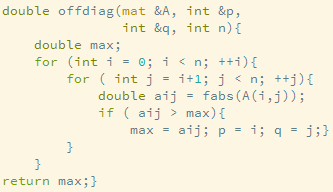
\includegraphics[width=0.47\textwidth]{C:/Users/sam61/OneDrive/Pictures/PHY480/Project2/1B_Offdiag.png}
	\label{uvx}
	\caption{Searches for largest off-diagonal element and saves the indices as p and q.}
\end{figure}

Jacobi rotate is the function acting as the similarity transformation from ${\mathbf A}$ to ${\mathbf B}$. It requires the indices found by offdiag as arguments so it knows which elements to change, but it does not initialize a rotation matrix and perform matrix multiplication. Rather, it takes the matrix ${\mathbf A}$ in as an argument and hard-codes the changes to its elements that matrix multiplication with rotation matrices would make.

\begin{figure}[!ht]
	\centering
	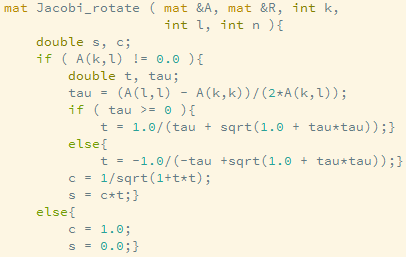
\includegraphics[width=0.51\textwidth]{C:/Users/sam61/OneDrive/Pictures/PHY480/Project2/2B_Jacobi_Rotate_1.png}
	\label{uvx}
	\caption{Part 1: ${\tau}$, tan, cos, and sin are initialized according to the methods shown in the algorithms section.}
\end{figure}

\begin{figure}[!ht]
	\centering
	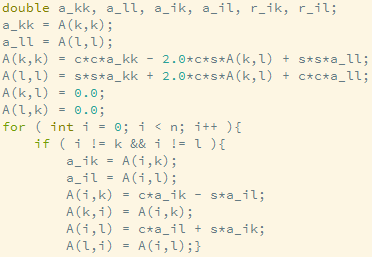
\includegraphics[width=0.47\textwidth]{C:/Users/sam61/OneDrive/Pictures/PHY480/Project2/3A_Jacobi_Rotate_2.png}
	\label{uvx}
	\caption{Part 2: The new, rotated elements of A are hard-coded in according to the algorithm.}
\end{figure}

The crux of the program is located in a while loop in the main body of the code, seen in figure 4. A few variables are declared outside of the figure. Tolerance is a number close to zero; in my case, 1E-10. An off-diagonal element is declared zero when its value falls below this "effective" zero. Once every off-diagonal element is zero, the loop terminates and the matrix is solved. The other while condition makes use of "iterations" and "maxiter". Iterations is simply a count of how many similarity transformations occur while the matrix is being solved, and maxiter limits the number of transformations in case the while loop runs away. Maxiter in my code is set to 100.

\begin{figure}[!ht]
	\centering
	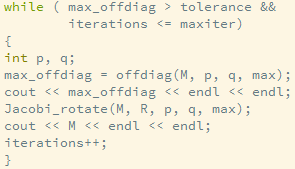
\includegraphics[width=0.40\textwidth]{C:/Users/sam61/OneDrive/Pictures/PHY480/Project2/5A_Jacobi_Method.png}
	\label{uvx}
	\caption{The while loop that performs successive rotations to the matrix.}
\end{figure}

Not shown in this report is the code that creates the initial matrix, but it can be found on GitHub.

	\subsection{Unit Tests}
To prove the accuracy of the code presented, I present two tests to ensure the mathematical soundness of the program. The first will be a simple demonstration of the function "offdiag". A 3 x 3 matrix with obvious non-zero off-diagonal elements is printed directly above the result of "offdiag". The second will demonstrate the preservation of orthogonality in the eigenvectors after one rotation, thus ensuring the transformation is unitary. The full code is on GitHub.

\begin{figure}[!ht]
	\centering
	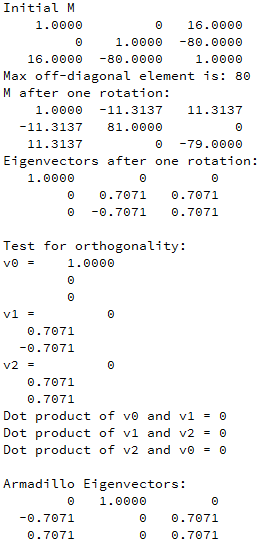
\includegraphics[width=0.40\textwidth]{C:/Users/sam61/OneDrive/Pictures/PHY480/Project2/Unit_Tests.png}
	\label{uvx}
	\caption{The output for both tests. You can see that in the initial matrix the largest off-diagonal element is -80, and positive 80 is returned as the output of "offdiag". In the remaining code, the post-transformation eigenvectors are shown. I took the dot product of them using an Armadillo method to show that they are still orthogonal. Lastly, I used an Armadillo method to calculate the eigenvectors as a double check that Jacobi Rotate made the correct eigenvectors after its single application.}
\end{figure}


\section{Results and discussions}
I will briefly explain my results, but for more specific images of the code output and actual data, visit my Github page: (\url{https://github.com/Sam617e/PHY-480-Work}).

I checked the eigenvalues that each algorithm gave against the eigenvalues that the Armadillo method "eig\_sym()" produced to see how accurate Jacobi's method was. Against my intuition, the diagonal of my final matrix always revealed the same numbers as the Armadillo method, to the extent of the decimal places that were visible to me (four, usually). This also did not depend on matrix size; My 4x4 matrix had agreeing eigenvalues, as did my 10x10. Also, for an inexplicable reason, my main code would not execute the while loop that rotates the matrix unless the matrix was printed out after each subsequent rotation. Although this did not affect the resulting eigenvalues, it did affect my opportunity to measure the time of "eig\_sym()" versus my algorithm. For the non-interacting case, I made a table of matrix sizes and iterations to complete the algorithm (${\rho_{max}}$ is fixed at 5, here) instead, to highlight their general relationship:

\begin{center}
	\begin{tabular}{cc}
		\hline \hline
			Matrix Size ($n x n$) &  Iterations\\
			\hline
			4 & 13\\
			6 & 39\\
			8 & 80\\
			10 & 101\\
			\hline
			\label{IterationTable}
	\end{tabular}
\end{center}
	
	As you can see, there is no discernible formula that will give the exact amount of iterations given a matrix's dimensions. However, it looks like it takes around $n^{2}$ iterations to completely diagonalize the matrix.

In the interacting case, the potential is changed and now has a term $\omega_{r}$ in it, the 'frequency' that reflects that strength of the oscillator potential. I plotted the wave function versus radius and varied $\omega_{r}$ to show how it affects the wave function.

	\begin{figure}[!ht]
	\centering
	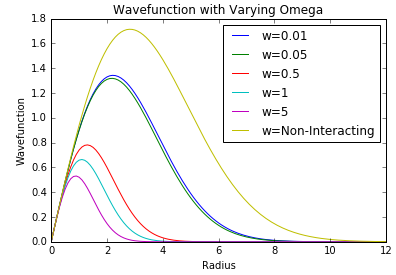
\includegraphics[width=0.525\textwidth]{C:/Users/sam61/OneDrive/Pictures/PHY480/Project2/WF_Plot.png}
	\label{}
	\caption{The wave function versus radius with varying $\omega_{r}$}
\end{figure}

Because $\omega_{r}$ is supposed to reflect the strength of the oscillator potential, it makes sense that a larger value would decrease the peak of the wave function. Should the oscillator potential be too strong, I can see the trend in this graph taking the wave function of these two electrons down to a value of zero.

I also took the interacting case, fixed $\rho_{max}$ at 5 and the matrix size at 8x8, and varied $\omega_{r}$ to see how the number of iterations were affected.

	\begin{center}
		\begin{tabular}{cc}
			\hline \hline
			$\omega_{r}$ & Iterations \\
			\hline		
			0.01 & 100  \\
			0.05  & 98 \\
			0.5 & 95 \\
			1 & 80 \\
			5 & 47 \\
			\hline
			\label{iterationsOmega}
		\end{tabular}
	\end{center}
	
Here, as well as at the previous table, a clear equation relating $\omega_{r}$ isn't obvious, but a general trend is clear. As the frequency increases in strength, the number of iterations decreases.

\section{Conclusions}
	Both the cases of one and two electrons trapped in a three-dimensional spherical potential were analyzed as eigenvalue problems and solved with Jacobi's method for diagonalizing matrices. I unexpectedly got a result that implied a degree of accuracy in the eigenvalues that rivalled the Armadillo method that is supposed to be more efficient. One case I considered as the root of this problem could be an issue where variables are stored in memory in a way such that the Armadillo eigenvalues printed off to me were actually the values on the diagonal of the final rotated matrix. 

Another, more vague suspicion I had was surrounding a quirk in the code I mentioned previously. For some reason, the algorithm would only proceed to apply rotations if the matrix was printed after each rotation (if not printed, it would stop after one transformation). It is possible this issue is tied to memory allocation and somehow affects my eigenvalues as well, but I am not sure how.

Unexpected results aside, it was shown that the number of iterations taken by Jacobi's method shrinks with the size of the matrix in the non-interacting case (and presumably in the interacting case as well). The number of iterations also shrinks with increasing values of $\omega_{r}$. Along with the increasing values of $\omega_{r}$ was a shrinking wave function, as seen in the plot, which makes sense physically given $\omega_{r}$ is a strength parameter for the oscillator potential.

	\subsection{Future Prospects}
	Solving the errors in the program noted above would be a good first step for a better analysis, as would more data points for the tables to make a more thorough argument. Also, as mentioned in the methods section, the offdiag function in the code could be optimized slightly further by not searching through the diagonal elements for the largest off-diagonal elements.

        \subsection{Acknowledgements}
        I am eternally grateful to Professor Morten Hjorth-Jensen for the C++ code examples that formed the backbone of this project, and also his unending patience and generosity when it comes to due dates. I would also like to thank John Bower for his scrutiny of my code for errors I did not end up resolving. Lastly, a special thanks to Parker Brue for aid on the wave function plots.

\begin{thebibliography}{9}
\bibitem{First}
M. Taut, Phys. Rev. A 48, 3561 (1993).
\bibitem{Second}
Hjorth-Jensen, Morten. "Computational Physics: Lecture Notes Fall 2015". Department of Physics, University of Oslo (2015).
\end{thebibliography}

\end{document}